\section{Stochastic Edge Acceptance}
After reading a lot about other models for evolving graphs I decided to come up with a new model for adding edges with an extra element of randomness.
The model is called Stochastic Edge Acceptance or SEA for short.
In most models the set of edges selected for evaluation are random but, but choosing which edge to add from that set is deterministic, like in the product rule where the one with the smallest product of cluster sizes is always accepted.

The underlying idea is to have a process which favors the minimization of the largest cluster through considering multiple edges at each step in the evolution algorithm, making it an Achlioptas process.
This is a local rule, i.e. it only considers local information such as the size of the clusters to which the nodes corresponding to the considered edges belong.
I wanted to create a simple probability using only the sizes of the clusters corresponding to the considered edges.
Using just the cluster size information it is easy to create a set of probabilities that decrease as the cluster size increases.
The way it is designed actually allows us to generalize this algorithm to evaluate $q$ edges at once with corresponding probabilities $p_i$, $i \in \{1, 2, ..., q\}$:

\begin{equation}
	p_i = \frac{\frac{1}{|C_i|}}{\sum_j \frac{1}{|C_j|}}
\end{equation}

A form of the algorithm for $q = 2$ can be written in pseudocode as follows:
\begin{itemize}
	\item Let $T$ be the total number of edges to add to the graph.
	\item Let $A_t = \{e_1, e_2, ..., e_t\}$ be the set of accepted edges at step $t$.
	\item Let $e_t^1$ and $e_t^2$ be the two nodes which edge $e_t$ would connect.
	\item Let $C(e_t^i)$ be the cluster which $e_t^i$ belongs to.
	\item Let $C(e_t) = C(e_t^1) \cup C(e_t^2)$ be the cluster which would be formed by activating $e_t$.
	\item Let $R \in [0, 1)$ be a randomly generated number.
\end{itemize}

\begin{algorithm}[H]
	\caption{Stochastic Edge Acceptance}\label{Stochastic-Edge-Acceptance}
	\begin{algorithmic}[1]
		\Procedure{SEA}{$T$}
		\State $A \gets \emptyset$
		\State $t \gets 1$

		\While{$t \le T$}
			\If{$C(e_t^1) = C(e_t^2)$}
				\State $A \gets A \cup \{e_t\}$
				\State $t \gets t+1$
			\ElsIf{$C(e_t'^1) = C(e_t'^2)$}
				\State $A \gets A \cup \{e_t'\}$
				\State $t \gets t+1$
			\ElsIf{$p$ > R}
				\State $A \gets A \cup \{e_t\}$
				\State $t \gets t+1$
			\Else
				\State $A \gets A \cup \{e_t'\}$
				\State $t \gets t+1$
			\EndIf
		\EndWhile
	\EndProcedure
	\end{algorithmic}
\end{algorithm}

The $q$-edge algorithm is similar except it would use a cumulative probability $P_i = \sum\limits_{j=1}^{i} p_j$ (much like in the $q$-state Potts model) and loop over $i \in \{1, 2, ..., q\}$ until $P_i > R$, and then once that is satisfied accept the edge and move to the next step.



%---------------------------------------------------------------------------------------
% Simulation and Analysis
%---------------------------------------------------------------------------------------
\section{Simulation and Analysis}
All data in this section was generated using \texttt{GraphEvolve.jl} (see Appendix \ref{ch:appendix} for more information).
Random networks of sizes $2^k$, $k \in \{15, 16, ..., 24\}$ were studied, and for each system size 1000 simulations were run with different random number generator seed values.
It would be ideal to run simulations for larger system sizes to get a more representative sample, and is something which can be investigated further in the future.
All code and the associated generated data used for this is publicly available on the corresponding GitHub page \url{https://github.com/cameronperot/explosive-percolation}.

Fig. \ref{fig:ER_BF_PR_SEA_transition} illustrates the order parameter of the SEA model in comparison with the ER, BF, and PR models.
The SEA model experiences a transition later than the ER and BF models, but before the PR model.
The order parameter shows a sharp increase at the point of phase transition with an almost vertical slope similar to that of the PR.

\begin{figure}[H]
	\centering
	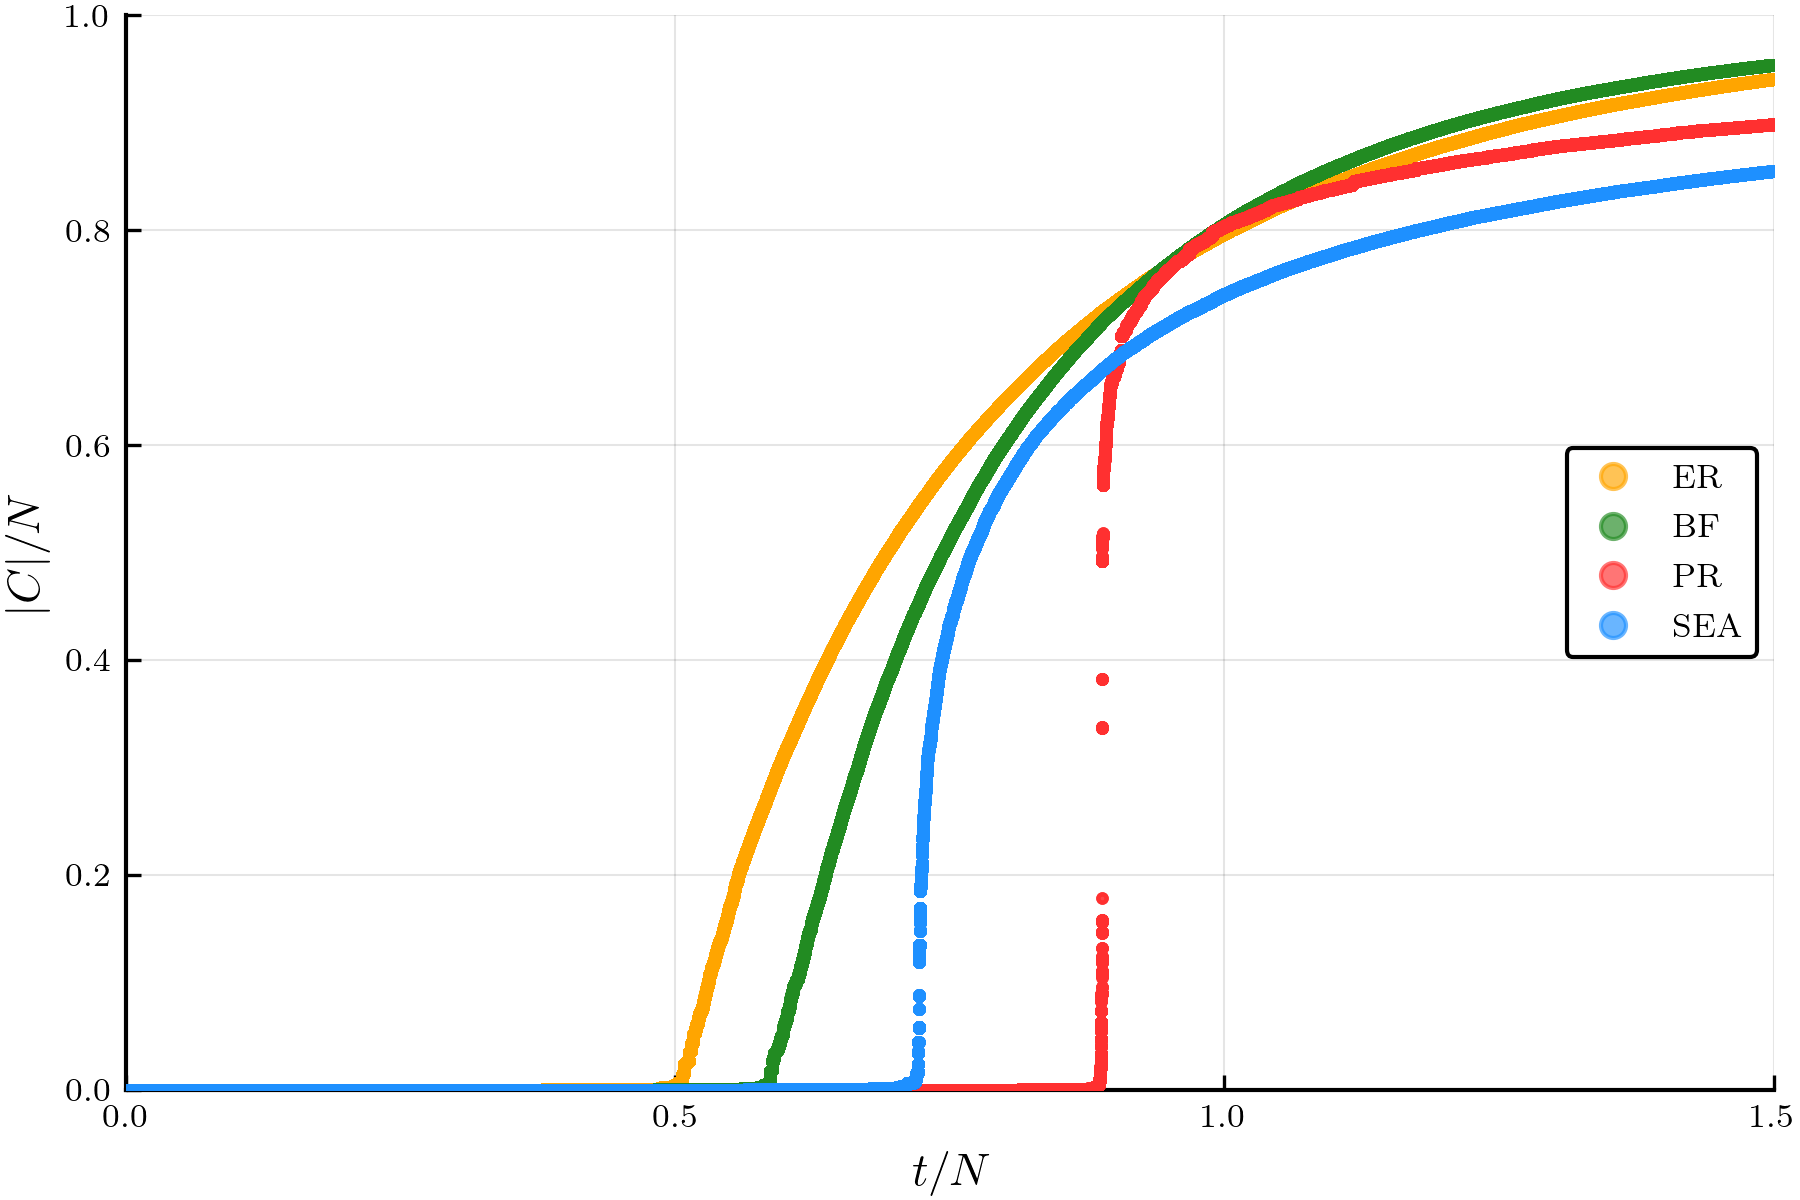
\includegraphics[width=350pt, clip]{images/Network_ER_BF_PR_SEA_1e6_order_param.png}
	\caption{Comparison of the stochastic edge acceptance order parameter to that of well-known models ER, BF, and PR. $N = 10^6$.}
	\label{fig:ER_BF_PR_SEA_transition}
\end{figure}

\begin{figure}[H]
	\centering
	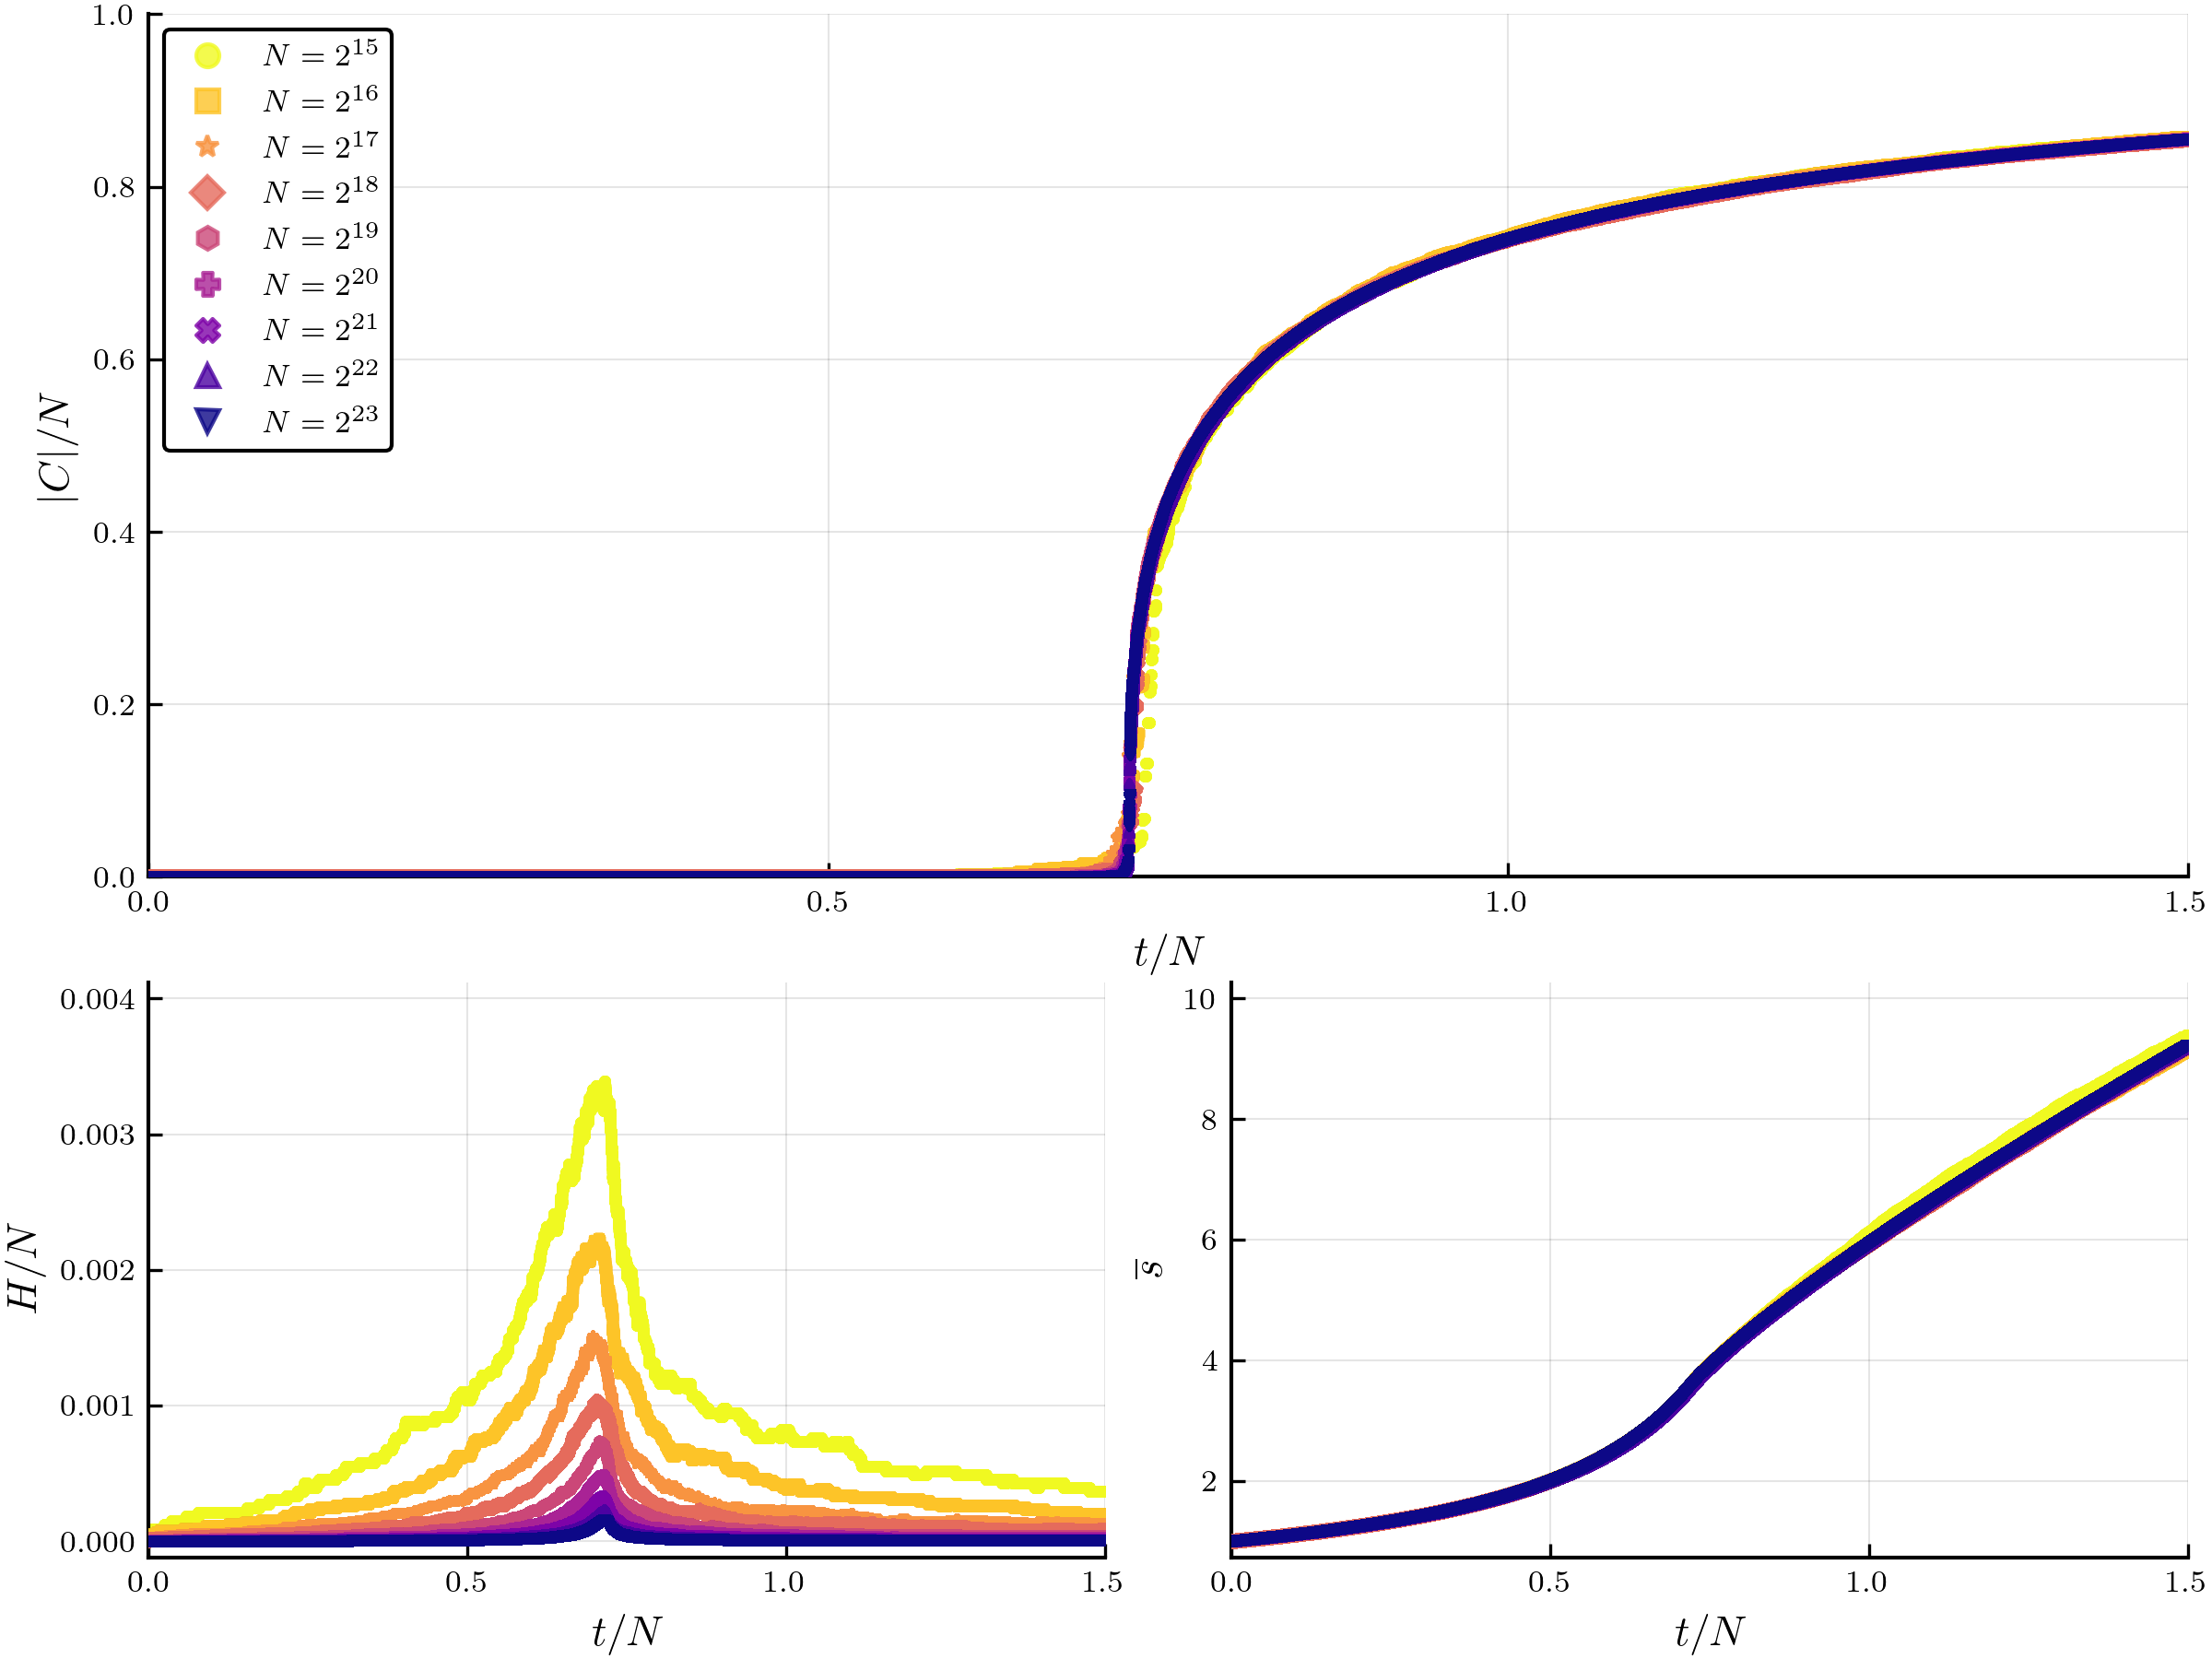
\includegraphics[width=350pt, clip]{images/k_scaling_triple.png}
	\caption{Observable dependence on system size. $H$ is the cluster heterogeneity and $\overline{s}$ is the average cluster size. As the system size increases the peak of the heterogeneity per node $H/N$ decreases and moves towards the right. The average cluster size lines up for all system sizes.}
	\label{fig:k_scaling_triple}
\end{figure}

Now that we've seen it exhibits interesting behavior at the point of phase transition we would like to learn more such as where does it transition, and most importantly, is it continuous?
In order to answer these questions we will use the framework laid out in \cite{Lee_1}.
First we need to find two points, one before the transition ($t_0$) and one after the transition ($t_1$).
We set $t_0$ as the step at which the cluster heterogeneity peaks, i.e. when the number of unique cluster sizes is at its highest.
We set $t_1$ as the step after the order parameter experiences its largest increase.
Let $r_i = t_i / N$ represent the relative number of edges in the system at step $t_i$ (because at step $t_i$ there are $t_i$ edges present in the graph), and $m_i = m(r_i)$ be the order parameter at step $t_i$.
We will define two quantities which we would like to study the behavior of:

\begin{equation}
\begin{split}
	\Delta r &= r_1 - r_0 \\
	\Delta m &= m_1 - m_0
\end{split}
\end{equation}

Fig. \ref{fig:r_scaling} shows the scaling behavior of $r_0$ and $r_1$ as a function of the system size $N$.
As the system size increases the two curves appear to be converging to the exact point of phase transition.
The obtained data tells us that the system transitions phases around $r \approx 0.718(4)$.

\begin{figure}[H]
	\centering
	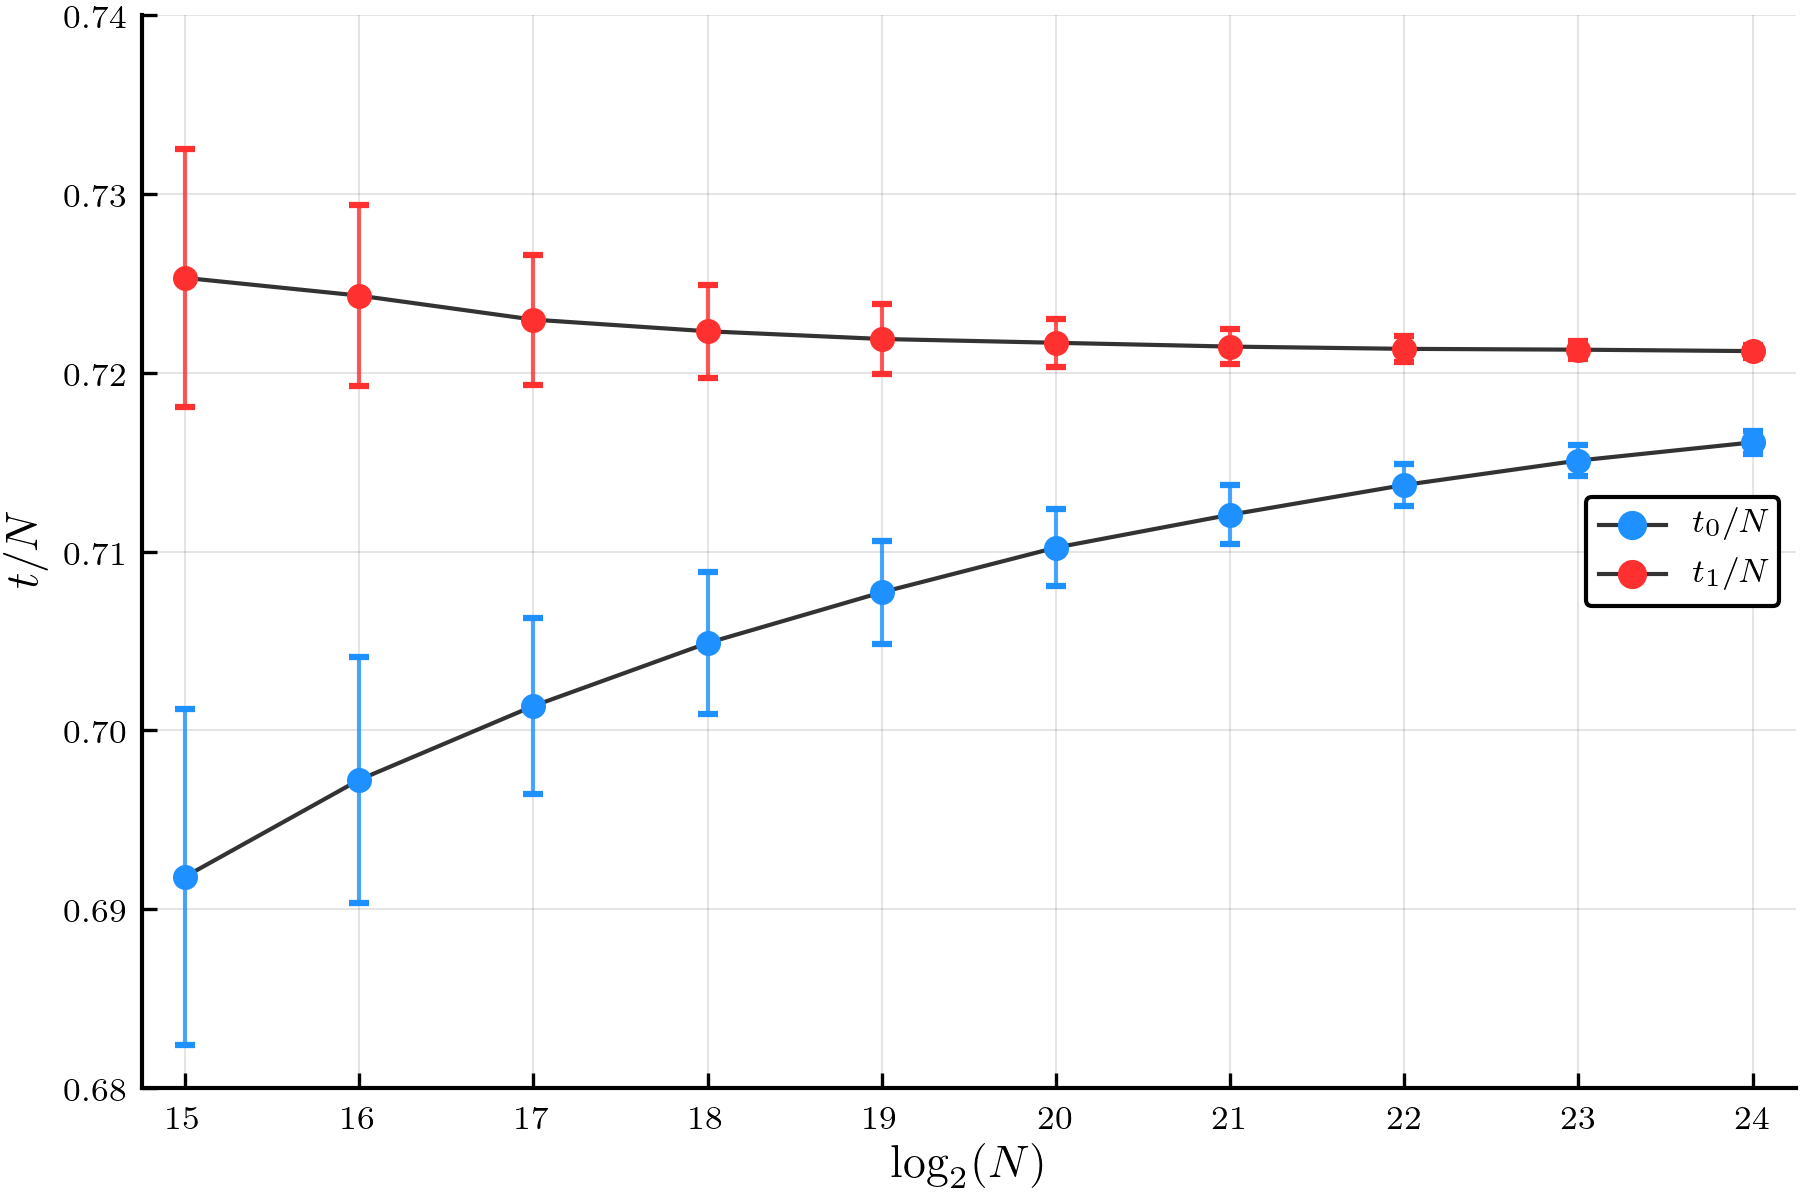
\includegraphics[width=350pt, clip]{images/r_scaling.png}
	\caption{The curves for $r_0$ and $r_1$ appear to be converging to the point of phase transition.}
	\label{fig:r_scaling}
\end{figure}

When looking at the scaling behavior of certain quantities it often helps to view them on $\log-\log$ plots to identify any power law scaling behavior.
Fig. \ref{fig:delta_r_scaling} shows $\Delta r$ as a function of the system size, and as we can see it exhibits power law scaling behavior of the form:

\begin{equation}
	\Delta r \sim N^{-\delta}
\end{equation}
with $\delta \approx 0.302(2)$.

\begin{figure}[H]
	\centering
	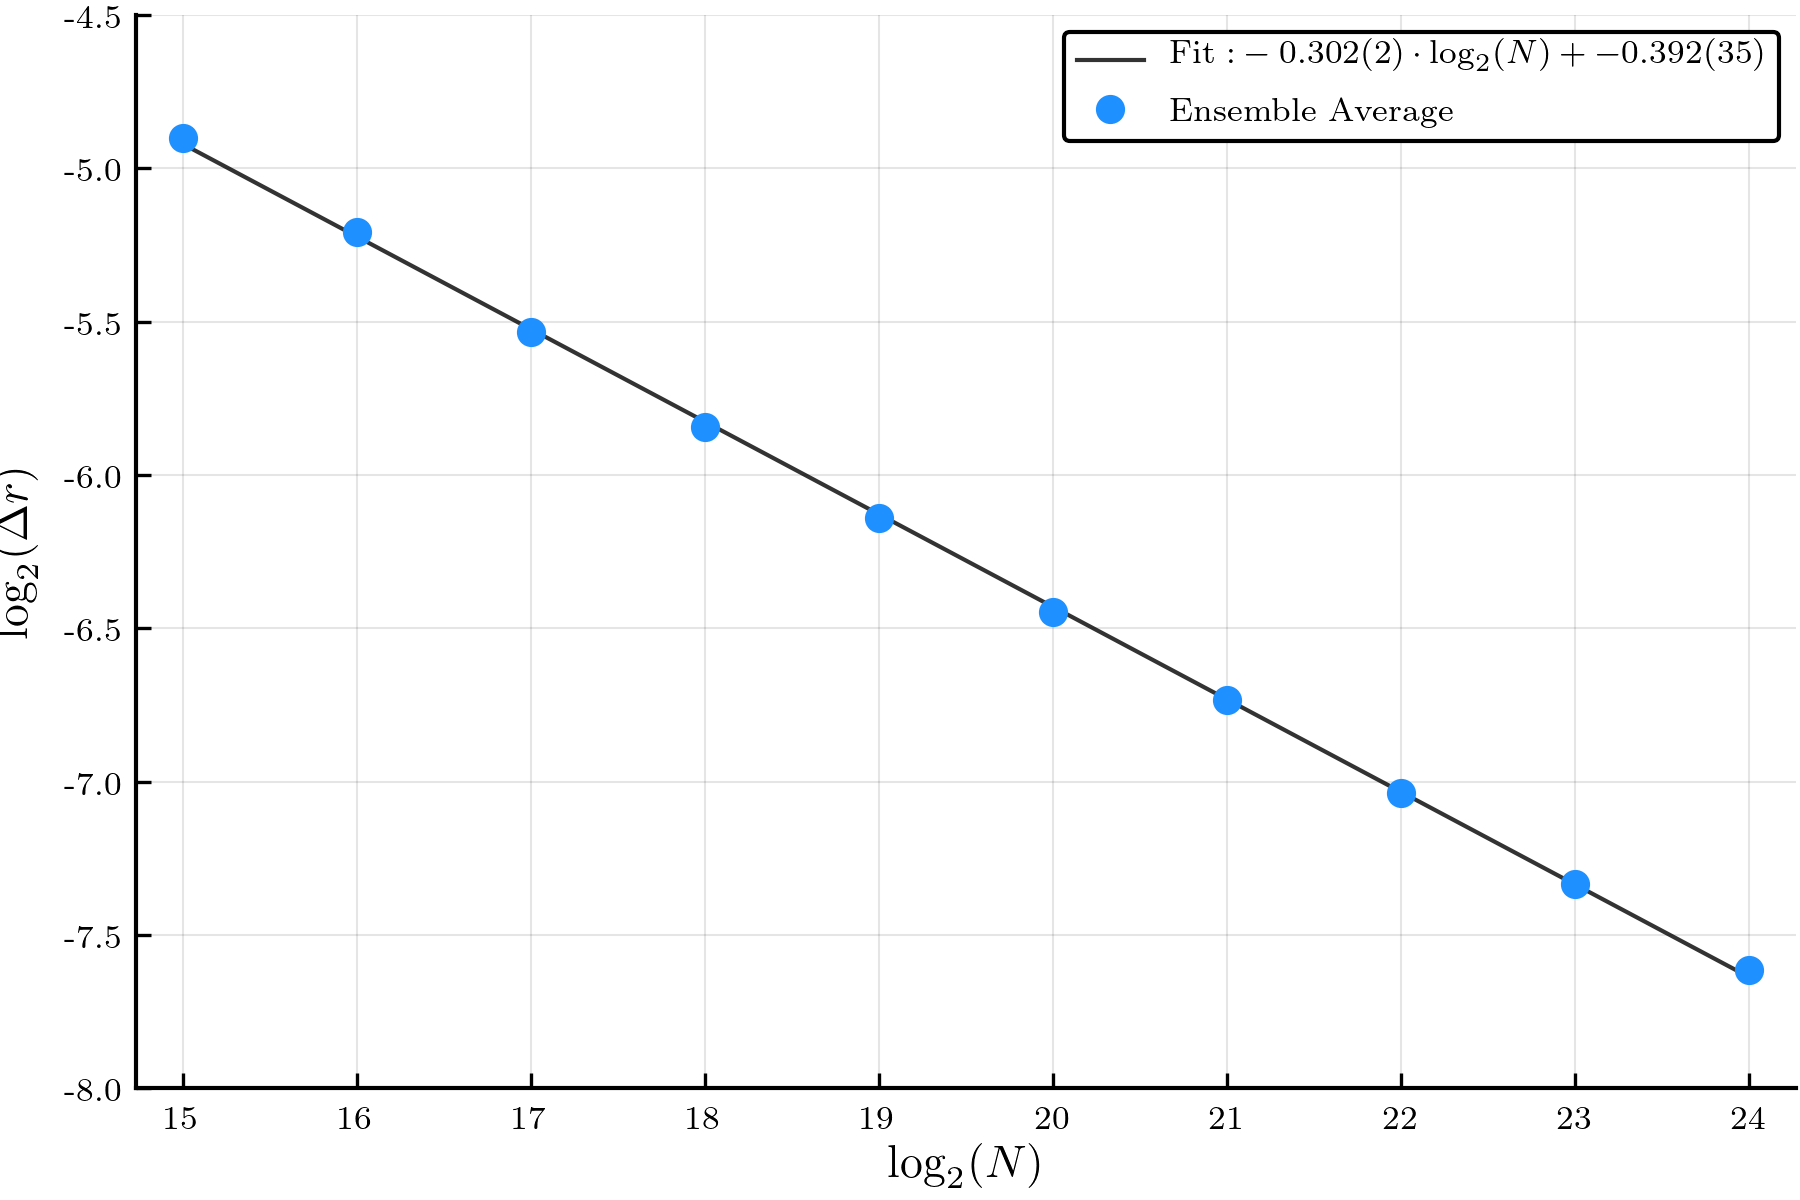
\includegraphics[width=350pt, clip]{images/delta_r_scaling.png}
	\caption{$\Delta r$ exhibits power law scaling in $N$.}
	\label{fig:delta_r_scaling}
\end{figure}

There is a lot of information contained in the cluster size distributions at $t_0$ and $t_1$.
We first start by analyzing the distribution at $t_0$, shown in Fig. \ref{fig:n_s_t_0}.

\begin{figure}[H]
	\centering
	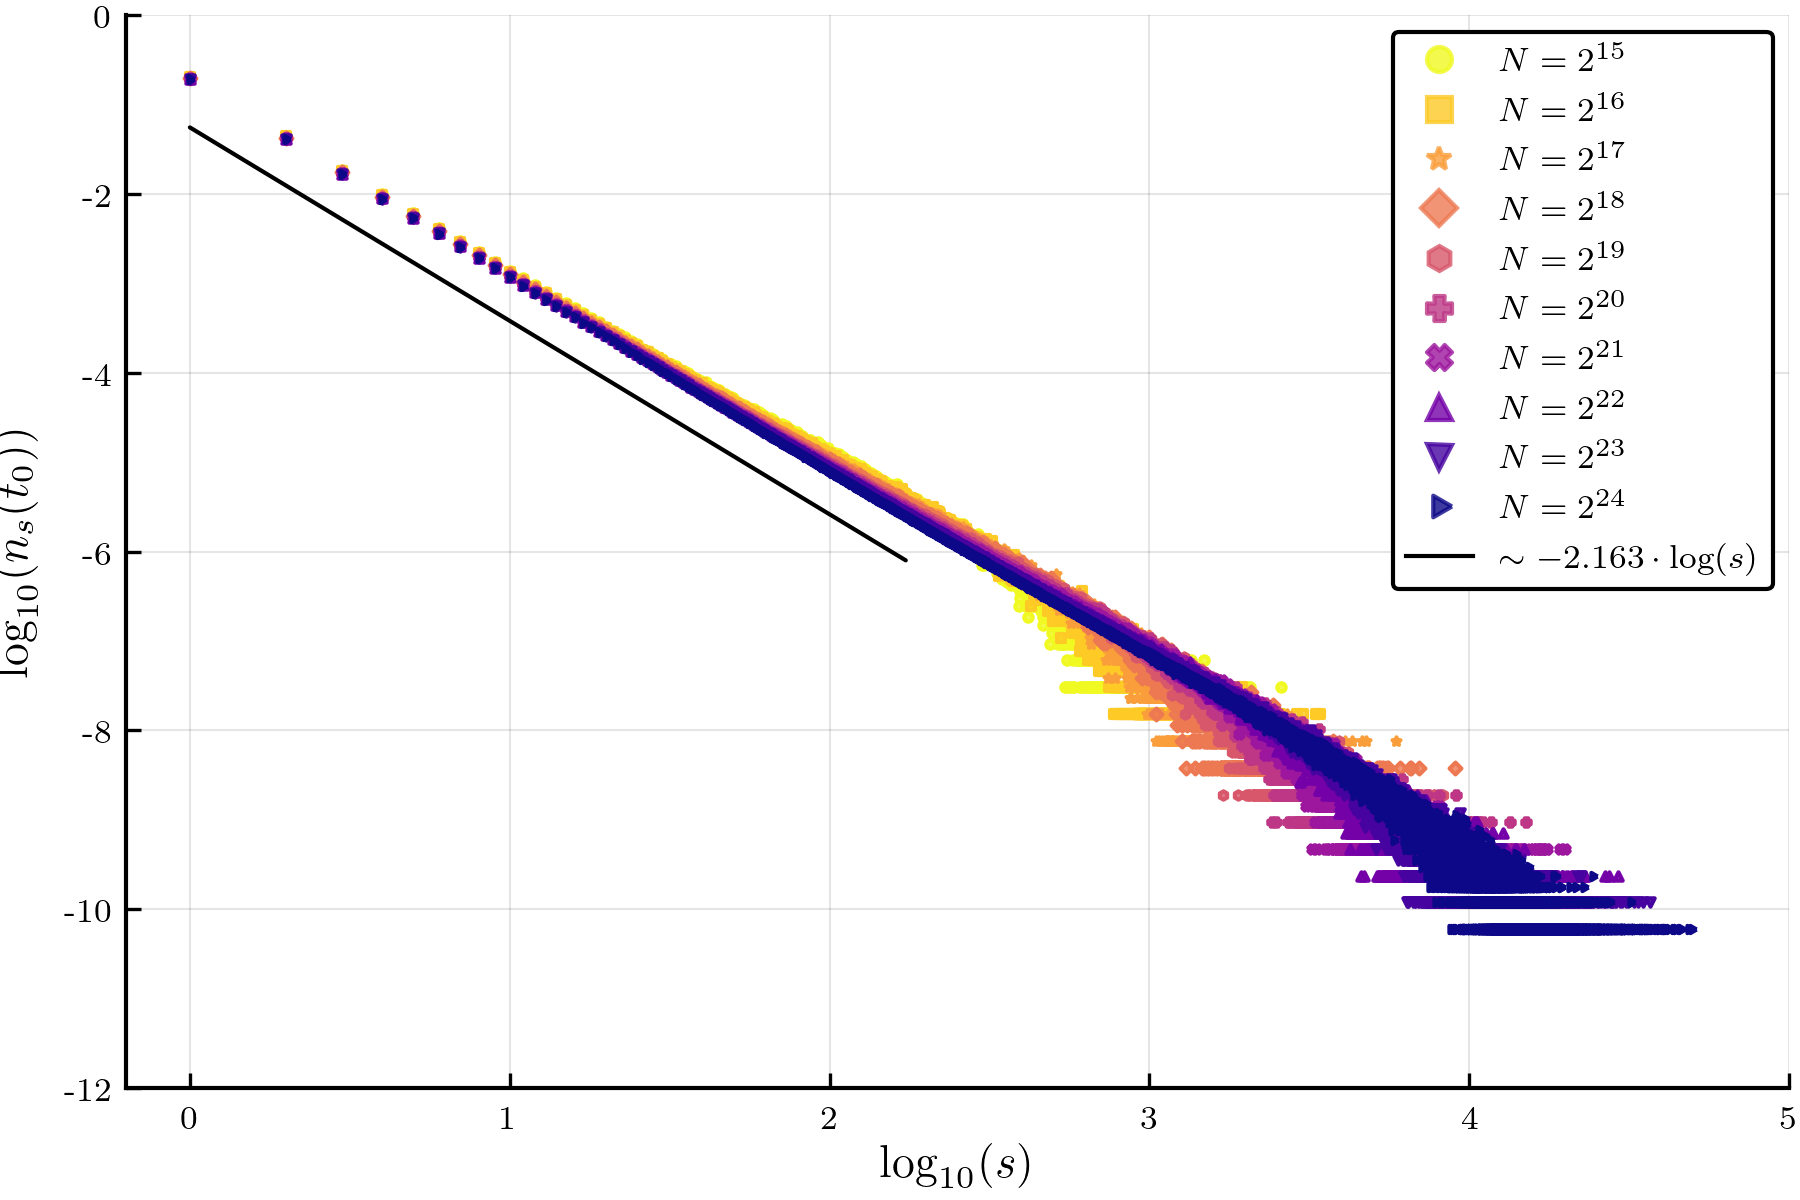
\includegraphics[width=350pt, clip]{images/n_s_t_0.png}
	\caption{Scaling behavior of the cluster size distribution at $t_0$.}
	\label{fig:n_s_t_0}
\end{figure}
When plotted on a $\log_{10}-\log_{10}$ basis we see a linear relationship up to a certain cutoff cluster size $s_f$ where $n_s(t_0)$ then drops off exponentially.
Large statistical errors are visible for higher values of $s$, but the overall message of the plot is clear.
This linear behavior tells us this is a power law in $N$ and using the ansatz:

\begin{equation}
	n_s(t_0) \sim s^{-\tau}
\end{equation}
and performing a linear fit gives us the value of the exponent $\tau_0 \approx 2.163$.

Looking at the data for the cluster size distribution at $t_1$ (Fig. \ref{fig:n_s_t_1}) we see a similar power law scaling relation, except with a slightly different exponent $\tau_1 \approx 2.218$.
I believe the discrepancy in the exponents here is due to the size of the simulations, and that if simulated with larger system sizes (such as up to $2^{37}$ seen in \cite{Lee_1}) that the values would converge towards the true value of $\tau$.
In Fig. \ref{fig:n_s_t_1} we see $\log_{10}(n_s(t_1))$ versus $\log_{10}(s/N)$ (rather than just $\log(s)$ as in Fig. \ref{fig:n_s_t_0}), where we again observe this linear scaling up to a point where it then dips and breaks the linear trend (again large statistical errors present past the cutoff point).

\begin{figure}[H]
	\centering
	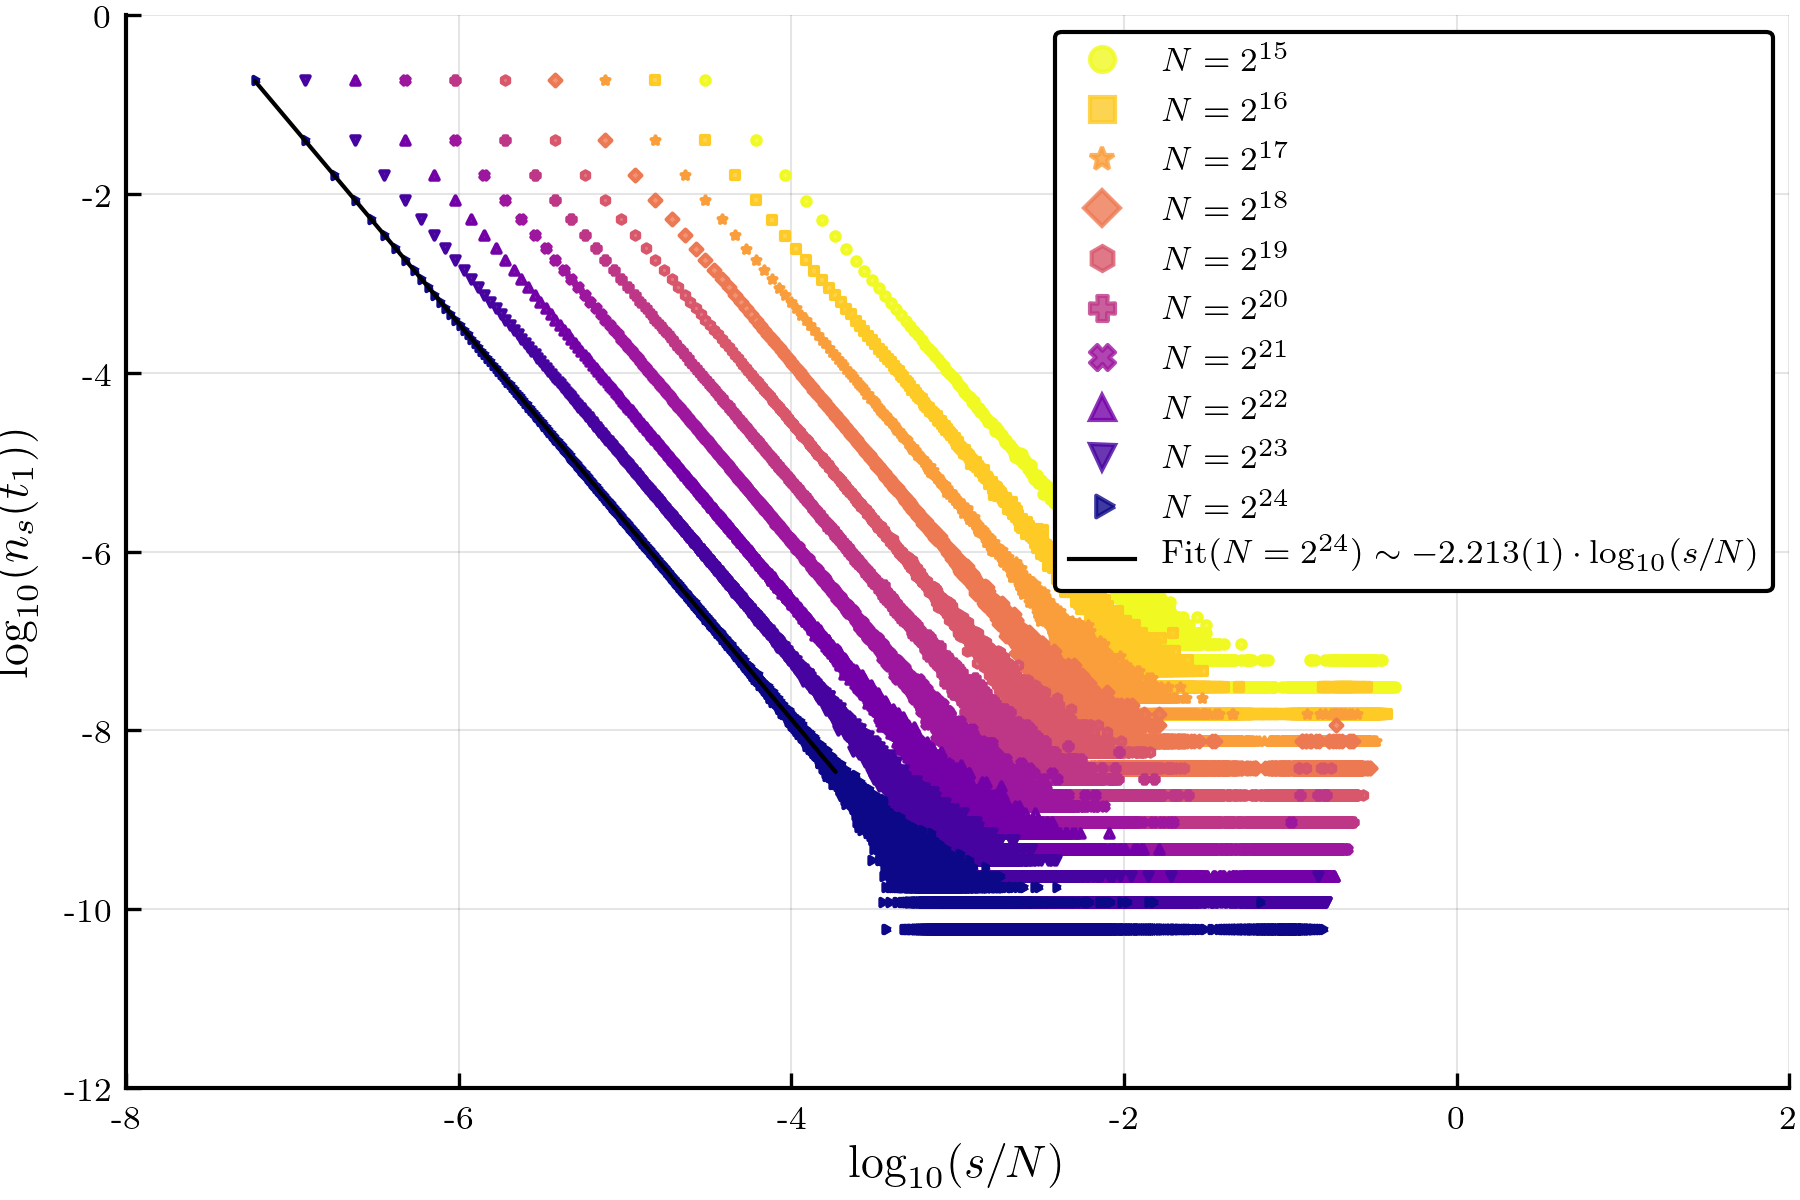
\includegraphics[width=350pt, clip]{images/n_s_t_1.png}
	\caption{Scaling behavior of the cluster size distribution at $t_1$.}
	\label{fig:n_s_t_1}
\end{figure}

In \cite{Lee_1} they determine $s_f$ by taking the ansatz $\sum_{s \ge s_f} \sim 1 / N_{C, 0}$ where $N_{C, 0}$ is the total number of clusters at $t_0$.
Then through the use of several relations such as the number of clusters scaling linearly with the system size they arrive at:

\begin{equation}
	s_f(N) \sim N^{1 / \tau}
\end{equation}

This can be verified by assuming a single characteristic cluster size and taking the finite-size scaling form of $n_s$ \cite{Lee_1}:

\begin{equation}
	n_s(t_0) = s^{-\tau} f(s / s_f) = s^{-\tau} f(s N^{-1 / \tau})
\end{equation}

Applying this same ideology to the stochastic edge acceptance method works quite well as seen in Fig. \ref{fig:fss_collapse_triple}, illustrating that the data for all of the system sizes lines up well and exhibits this hump behavior also seen in \cite{Lee_1}.
This verifies that indeed $\tau_1 \approx 2.218$ is a good estimation of $\tau$.
The data analysis up to this point leads me to believe that the discrepancies in the fitted values of $\tau$ could be due to $t_1$ being closer to the critical point than $t_0$, and as $N$ increases we see $t_0$ move closer to $t_1$ (Fig. \ref{fig:r_scaling}), thus if we ran simulations with larger values of $N$ then we should be able to obtain a more accurate reading of $\tau$.

\begin{figure}[H]
	\centering
	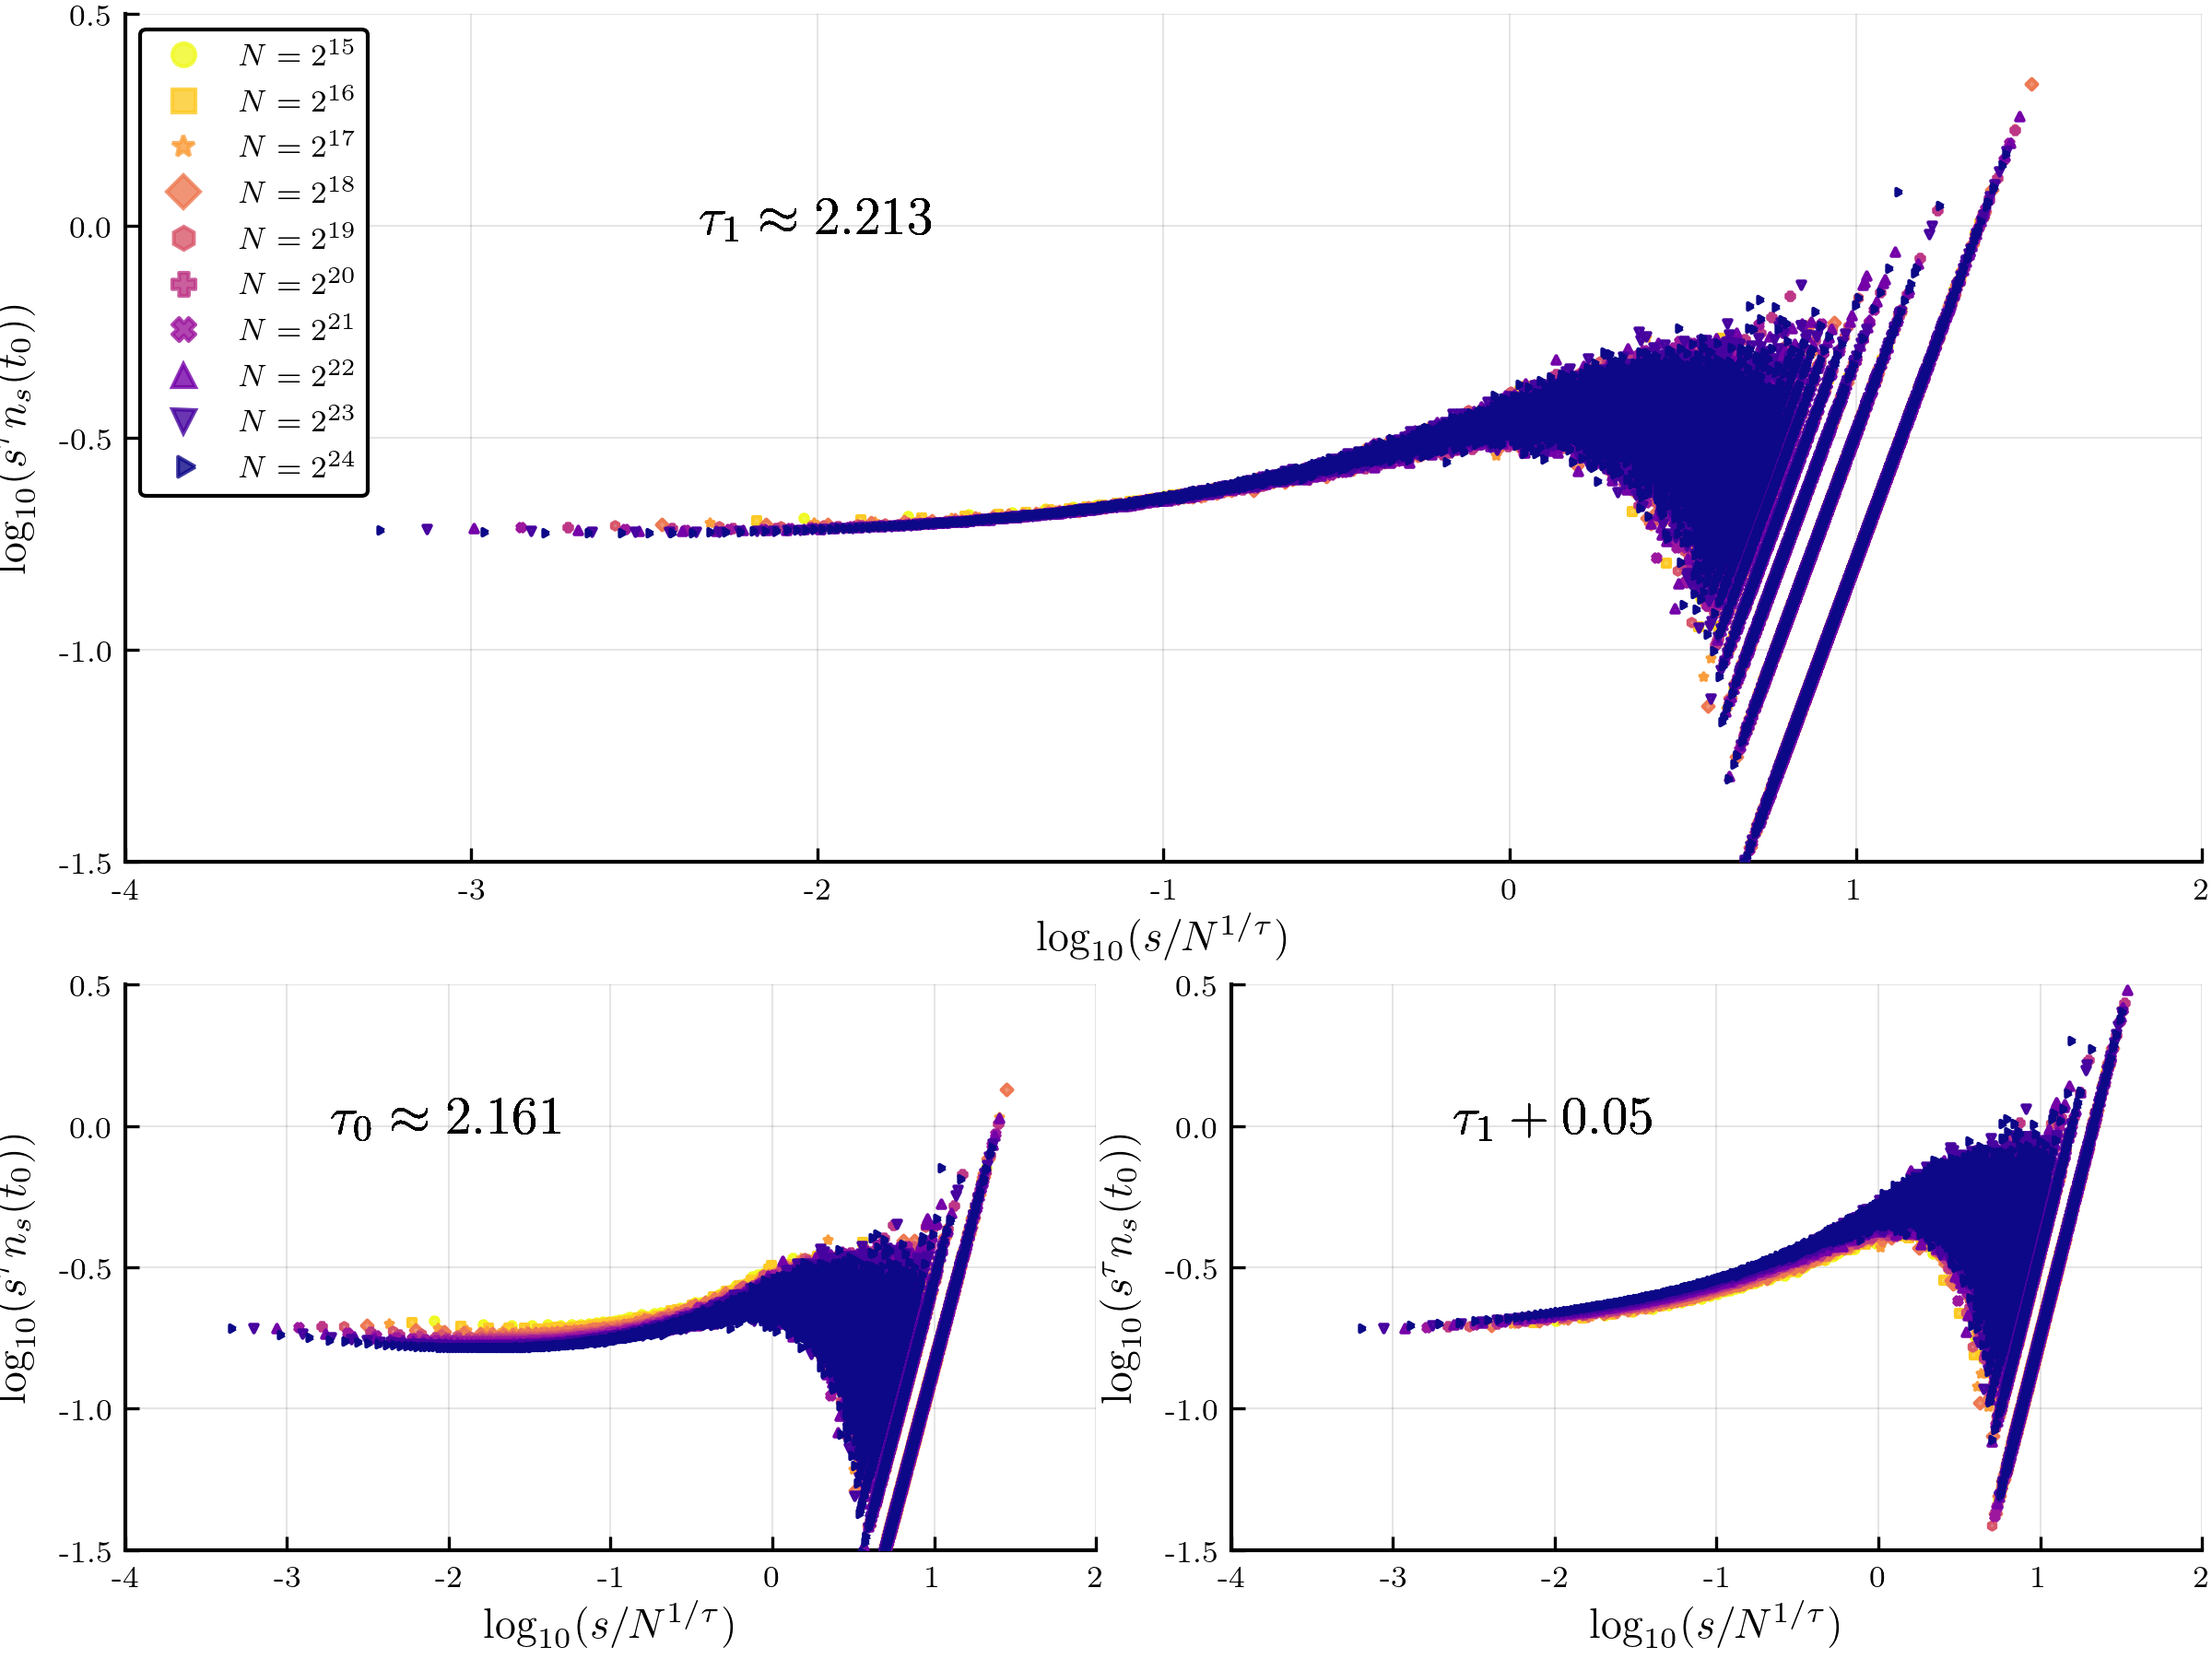
\includegraphics[width=350pt, clip]{images/fss_collapse_triple.png}
	\caption{$n_s(t_0)$ finite-size scaling shows a collapse of the data for the critical exponent value $\tau_1 \approx 2.218$ obtained from fitting the linear portion of the distribution at $t_1$. The lower left plot shows how the collapse looks for the value $\tau_0$ and the lower right plot illustrates a slightly higher value of $\tau$, both of which do not line up as well as when using $\tau_1$.}
	\label{fig:fss_collapse_triple}
\end{figure}

Now that we have extracted some useful information, namely the values of the critical exponents, we want to show that as the system size tends to infinity, the difference in the order parameter, $\Delta m$, tends to zero (i.e. $\lim_{N \rightarrow \infty} \Delta m = 0$).
In order to show this we want to place an upper bound on $\Delta m$. In \cite{Lee_1} they laid out a clever method for setting an upper bound by starting with the cluster size distribution at $t_0$ and taking an ideal process to add edges in such a way as to maximize the largest cluster size from $t_0$ to $t_1$, thus any other process will produce a $\Delta m$ that is bounded above by the $\Delta m$ produced in the ideal process.
This ideal process would seek to merge all clusters larger than some size $s_\delta$, which is determined by $\Delta t = t_1 - t_0$ and the cluster size distribution at $t_0$, i.e. $\Delta t = N_{C, 0} \sum_{s > s_\delta} n_s(t_0)$, where $N_{C, 0}$ is the total number of clusters at step $t_0$.
What they arrived at is that \cite{Lee_1}:

\begin{equation}
	\Delta m \lesssim s_\delta^{2 - \tau} \sim N^{-\delta (\tau - 2) / (\tau - 1)}
\end{equation}

Plugging in our obtained values of $\delta$ and $\tau$ we find that $\Delta m \lesssim N^{-0.056}$, which implies that the transition of the stochastic edge acceptance model is continuous like other local information based models.
Fig. \ref{fig:delta_m_scaling} shows $\log_2(\Delta m)$ versus $\log_2(N)$ and fitting a line we observe a decay exponent of $0.152(2)$ and verify that this is indeed below the upper bound we arrived at.

\begin{figure}[H]
	\centering
	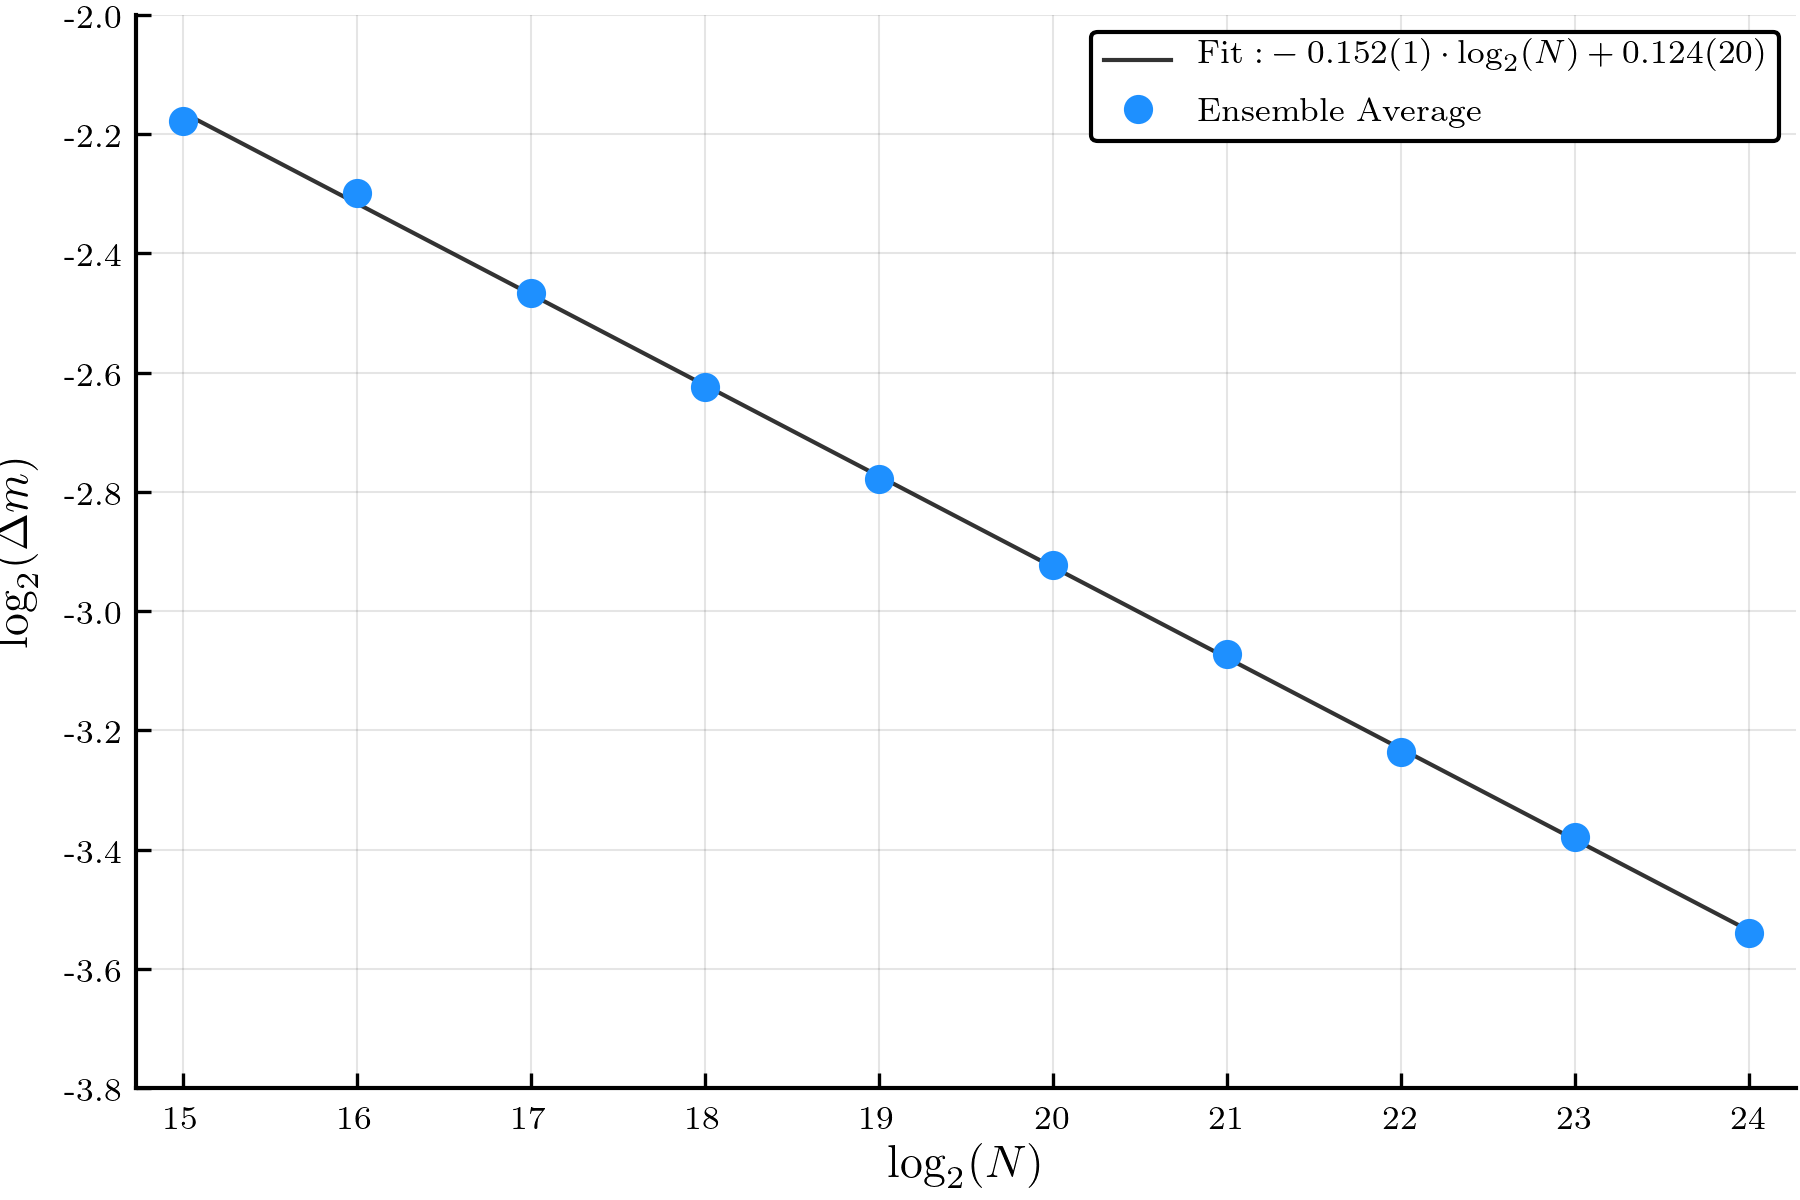
\includegraphics[width=350pt, clip]{images/delta_m_scaling.png}
	\caption{Plotting the change in the order parameter versus the system size on a $\log_2-\log_2$ scale shows that it is well below the upper bound we determined.}
	\label{fig:delta_m_scaling}
\end{figure}



%---------------------------------------------------------------------------------------
% Possible Future Directions
%---------------------------------------------------------------------------------------
\section{Possible Future Directions}
There are many different avenues we could go down in the future to further the analysis presented here and in the referenced sources.
The most obvious are studying $q$-edge models for $q \ge 3$ and seeing how the system behaves as $q$ changes, as well as looking at systems other than random networks, such as a lattice.
As a sneak peak, the Figs. below illustrate how the order parameter changes in these scenarios.

Fig. \ref{fig:q_scaling_triple} shows the order parameter for systems of size $N = 10^6$ and $q \in \{2, 3, ..., 7, 8\}$. As we can see, increasing the number of edges evaluated delays the transition even longer, which makes sense from a practical standpoint since more candidate edges means we have more opportunities to minimize the size of the largest cluster.

\begin{figure}
	\centering
	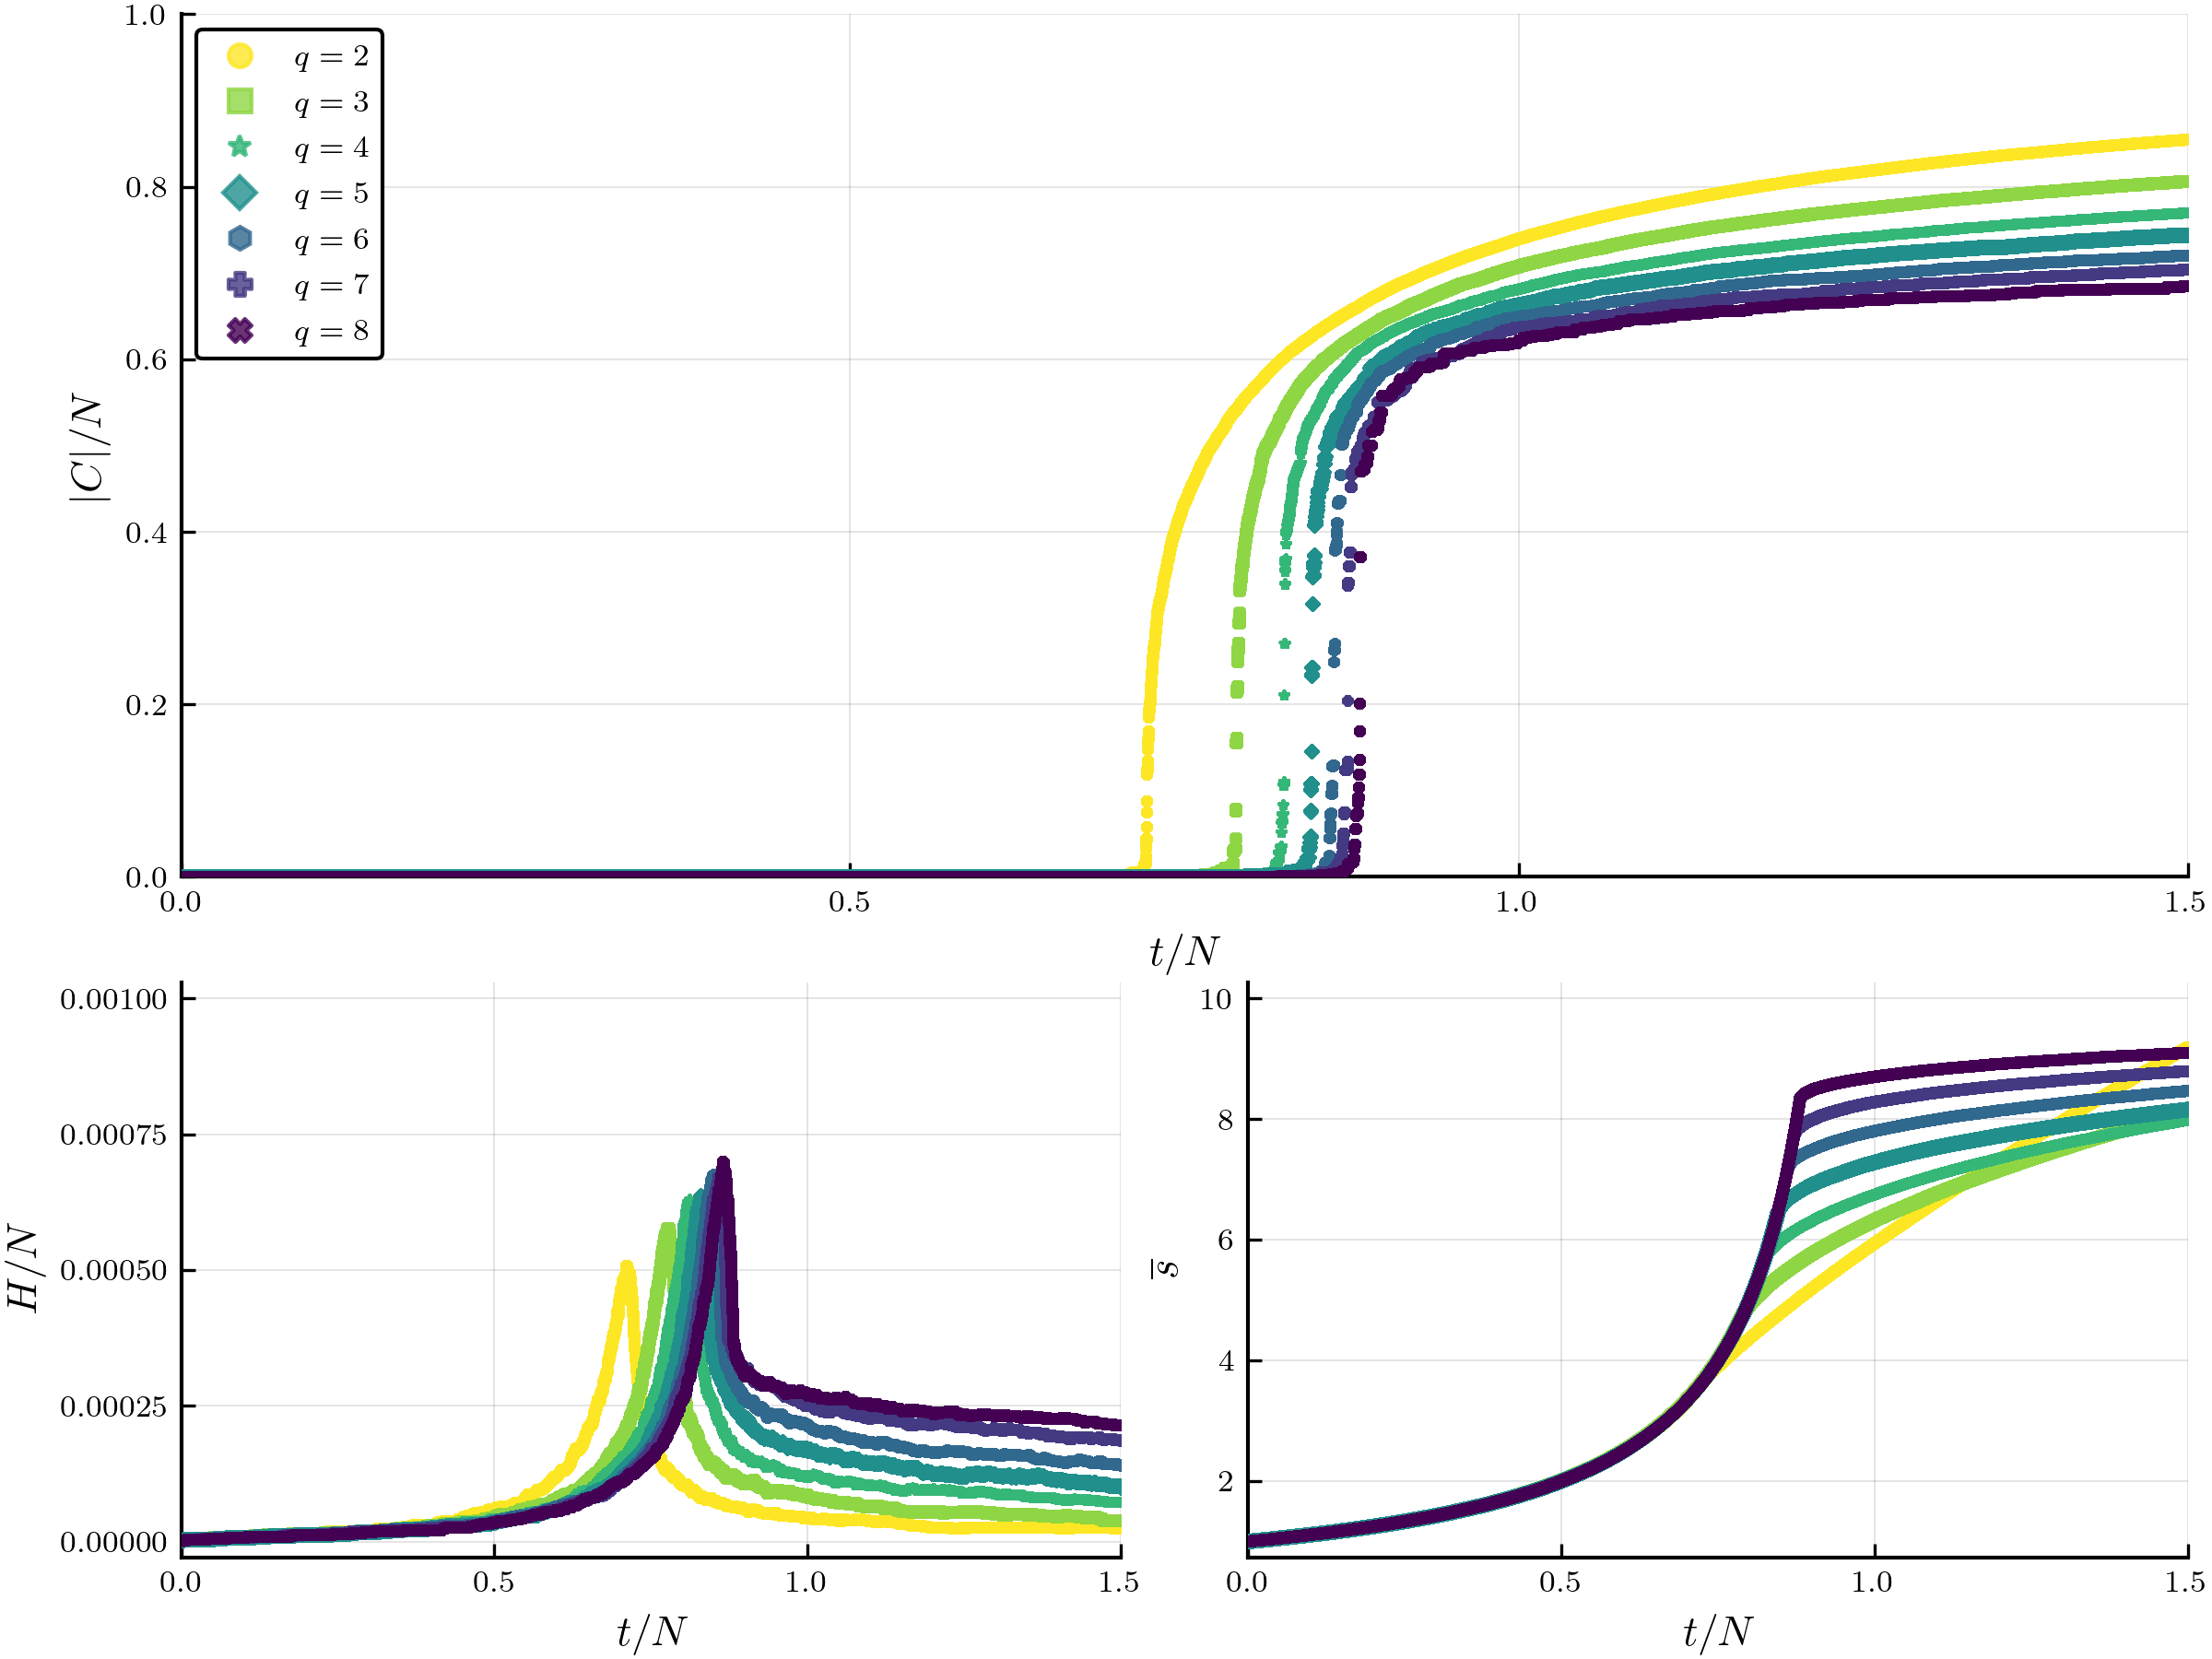
\includegraphics[width=350pt, clip]{images/q_scaling_triple.png}
	\caption{Stochastic edge acceptance model dependence on $q$. As $q$ increases we see the transition is delayed even longer. The heterogeneity per node exhibits sharper peaks, and the average cluster size shows interesting behavior. $N = 10^6$.}
	\label{fig:q_scaling_triple}
\end{figure}

Fig. \ref{fig:Lattice2D_ER_BF_PR_SEA_transition} illustrates what happens when we change the graph type to a 2D square lattice allowing only edges between nearest neighbors.
We see that doing so shifts order parameter to a later point, which makes sense due to the fact that on a two dimensional lattice each point only has four neighbors thus only four possible edges it can be connected with.

\begin{figure}[H]
	\centering
	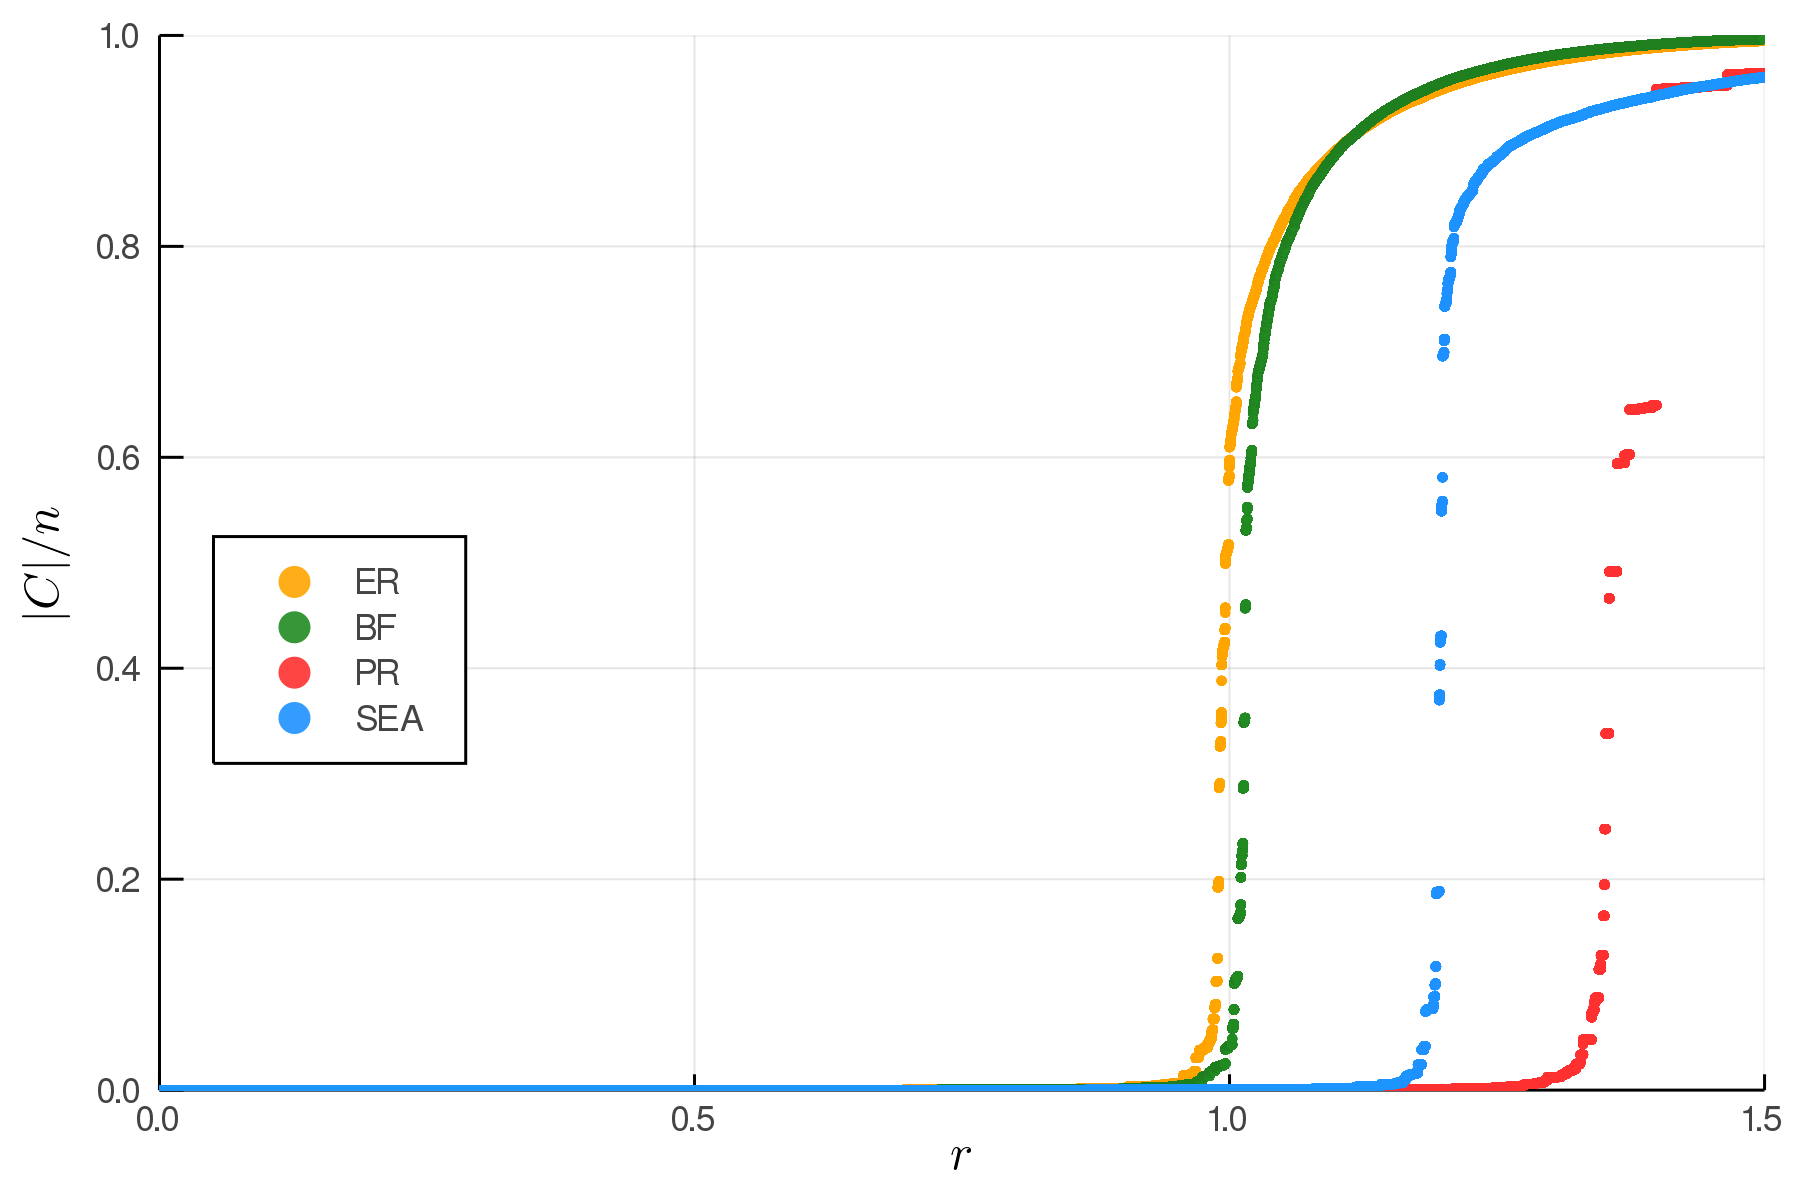
\includegraphics[width=350pt, clip]{images/Lattice2D_ER_BF_PR_SEA_1e6_order_param.png}
	\caption{Stochastic edge acceptance model order parameter when run on a 2D square lattice. $L = 10^3$.}
	\label{fig:Lattice2D_ER_BF_PR_SEA_transition}
\end{figure}

Fig. \ref{fig:Lattice3D_ER_BF_PR_SEA_transition} illustrates the case of allowing only nearest neighbor edges on a 3D cubic lattice. The transition is delayed longer than that in a random network but is before that on a 2D lattice, which again makes sense because now we have six neighbors with which we can activate edges between.

\begin{figure}[H]
	\centering
	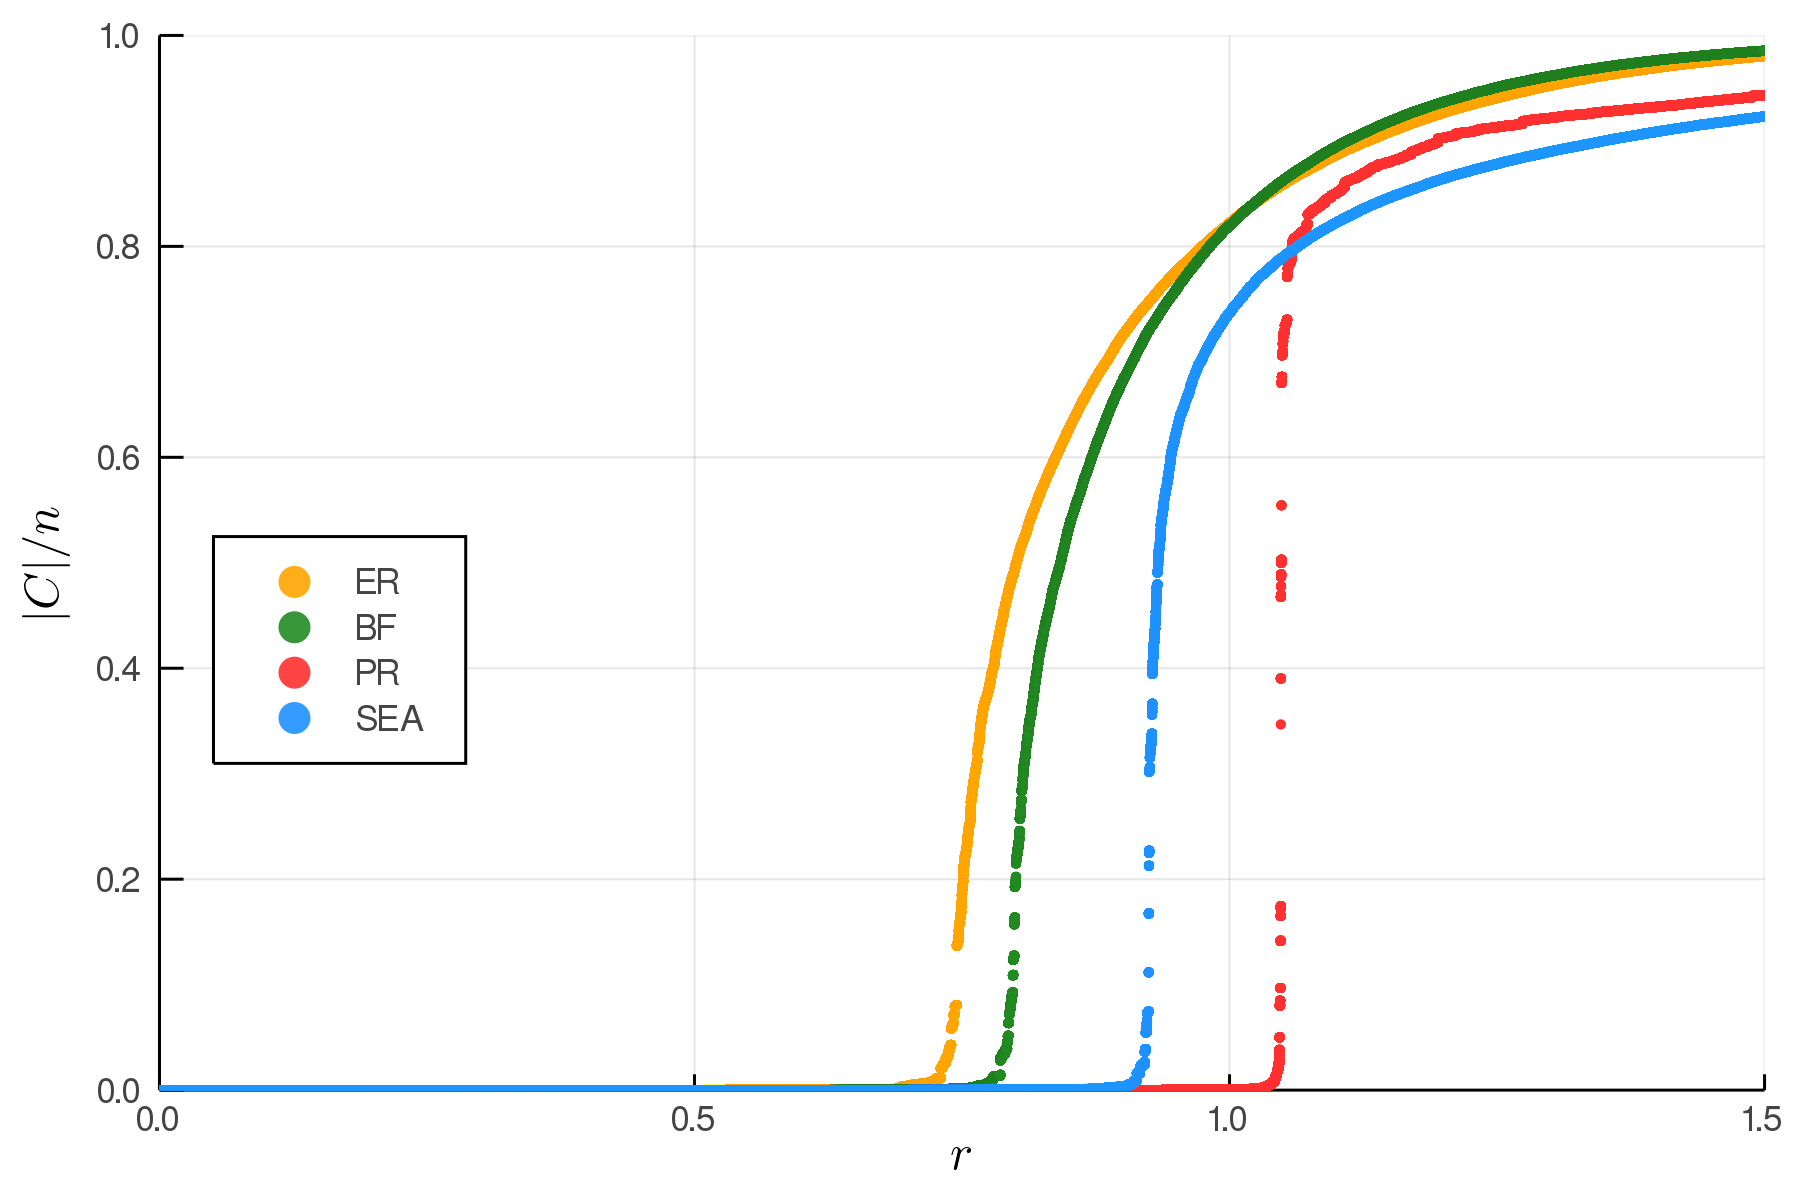
\includegraphics[width=350pt, clip]{images/Lattice3D_ER_BF_PR_SEA_1e6_order_param.png}
	\caption{Stochastic edge acceptance model order parameter when run on a 3D cubic lattice. $L = 10^2.$}
	\label{fig:Lattice3D_ER_BF_PR_SEA_transition}
\end{figure}
